--> Je Subsection Punkt Fragen formulieren.

\section{Theoretische Grundlagen}
	\subsection{Problemstellung}
	
	Es gibt zwei grundlegende Probleme die eine PL/I zu Java Übersetzung lösen soll. 
	
	Einerseits das Kompatibiltätsproblem von PL/I-Programmen, die auf modernen Platformen laufen sollen, wie etwa Cloud-Instanzen, oder Linux-Server. Andererseits die mit einem hohen Aufwand verbundene Wartung von bestehenden PL/I-Programmen. 
	
	Bestehende PL/I Compilerlösungen führen aktuell zu einem Kompatibilitätsproblem. Der PL/I Compiler, der auf den meisten Computer-Systemen im Einsatz ist wird von IBM entwickelt und vermarktet. Hierbei handelt es sich um einen Compiler der expilziet für z/Os geschrieben wurde. Dabei ist z/Os ein Betriebssystem für die von IBM vermarkteten Großrechner. Eine kompilierung von PL/I auf einem herkömmlichen x86-Desktop Computer oder in der Cloud ist mit diesem Compiler nicht möglich. 
	(https://www.ibm.com/de-de/products/pli-compiler-family) 
	Eine Alternative bietet die Organisation GNU mit der GNU Compier Collection (GCC). Der Entwickler Henrick Sorensen entwickelte Teile des Frontends für einen PL/I Compiler. Dabei verwendete er das Backend, das die GCC zu verfügung stellt. Jedoch gab es bei diesem Projekt seit 2007 keine weiteren Neuerungen mehr. Der Entwickler gibt an, das bisher keine Zwischencode Erzeugung stattfindet, was diesen Compiler bisher unbrauchbar macht. Somit ist dieser Compiler keine Alternative zu dem von IBM.
	(https://pl1gcc.sourceforge.net/) 
Es bleibt bisher also nur die Möglichkeit über einen Emulator PL/I-Code auf einem z/Os System zu kompilieren.

Weiterhin ist PL/I eine Altsprache, die seit den 1960er Jahren im Einsatz ist. 

(https://www.fruehes.berlin/wp-content/uploads/2011/02/PL-1-F-OS-360-V-4.0.pdf, erste Seite) 

Es ist also anzunehmen das diese Sprache heute zwar noch in Computer-Systemen zu finden ist, aber der Bestand an Entwicklern die PL/I-Software Warten können vermutlich gering ist. Wartung und Entwicklung werden so häufig schwer und teuer.

Java hingegen ist auf nahezu allen erdenklichen Systemen Kompilierbar, durch die Systemunabhängig Java Virtual Machine (JVM). 

(https://medium.com/@etherservices.vimalraj/can-i-run-java-programs-on-any-device
a-comprehensive-guide-31f736ca6ab1) 

Dabei sind die Programme auch mit Android-Systemen kompatibel, die einen weitaus weniger Komplexen RISC Befehlsatz als x86-Systeme mit einem CISC Befehlssatz haben.

(https://developer.android.com/codelabs/build-your-first-android-app) 
Zusätzlich ist eine Kompilierung auch auf einem IBM-Großrechner möglich. 

(https://www.ibm.com/docs/en/zos-basic-skills?topic=zos-java)

Das macht Java zu einer flexibel Einsetzbaren Sprache. Weiterhin is Java die mit am meisten verwendete Programmiersprache in der heutigen Zeit. (Quelle?) Das führt zu einer höheren Anzahl an Entwickler, die in der Lage sind Java Programme zu warten.

% Was ist ein Transpiler?
Um nun Java für die Lösung der dargelegten Probleme zu verwenden, wird ein Programm benötigt, welches PL/I Quellcode in Java Quellcode übersetzt. Ein solches Programm verarbeitet PL/I-Code so, dass aus diesem Java-Code generiert werden kann. Dabei ist es möglich das der Entwickler des Programms, selbst wählt wie er welche Ausdrücke übersetzt. Ist der Programmcode erstmal in Java übersetzt worden, kann dies durch die JVM kompiliert werden.

Am Ende ist zwar der Quellcode übersetzt und auch kompilierbar, jedoch ist erst ab diesem Punkt die tatsächliche Qualität des Programms zu erkennen. Faktoren wie Lesebarkeit und Erweiterbarkeit des übersetzen Programmcodes gehen in die Beurteilung mit ein. 
Die Beurteilung der Qualität des Programms ist auch von Zielaspekten der Benutzer abhängig. Für das zu entwickelnde Übersetzunsgporgramm, wurden Zielgruppen definiert die im nachfolgenden Kapitel 1.2 weiter erläutert werden sollen. Diese Zielgruppen sind für weitere Gestaltungsentscheidungen in der Entwicklung des Programms wichtig.

%Anderseits auch die veränderte Laufzeit-Performance. Die Laufzeit-Performance kann durch eine Übersetzung verschlechtert, wie auch verbessert werden. Somit ist nicht nur die reine Übersetzung Teil der Problemstellung, sondern es gilt auch die Übersetzung zu beurteilen. 
\pagebreak
     
% Cross Compiler? - Hat hier eig nix zu suchen, ist Thema für Boostrapping aber nicht für Transpiler
     
     
     
% 	 Welches Problem löst das Programm?
%	 Probleme 
%			 1. Nicht auf jedem System läuft PL/I, besonders nicht auf modernen x86 bzw. Cloud.
%			 2. PL/I ist eine weniger verwendete Sprache, Wartung teuer &  Schwer.

%	 (Hinführung zum Problem:
%	 Historisches Kompatibilitätsproblem -> Nicht auf jedem System lief jede Assambler Sprache, Problem: hoher Aufwand und Unflexibel
% 	 Deshalb -> Compiler mit Hochsprache, der Code für das Backend des Compilers, bspw. C's Gcc Compiler
%    in Assambler Sprache des Systems übersetzt.)? **Hier einen Cross Compiler erklären bzw. im Zusammenhang mit dem Historischen Problem.**

%	 Problem mit PL/I -> Pl/I Compiler rar bzw. nur für Großrechner Systeme vorhanden   
%	 Es gibt zwar einen GCC Pl/I Compiler, dieser wird aber seit 2007 nicht mehr weiterentwickelt. Eine Weiterentwiclung könnte auch Interessant %    sein, löst aber nicht das Problem der teuren Wartung von Programmen in PL/I.

% 	 
%	 Lösungsvorschlag zu 1 -> PL/I zu Java Transpiler bauen Java und JVM relativ System unabhängig und damit Ideale Zielsprache für eine 
%	 hohe Kompatibiltätsrate.Um zum Beispiel Pl/I Programm die auf einem Großrechner laufen auch auf einem x86 On-Prem Server oder einer Cloud
%    zu betreiben. **Hier die Frage klären was ein Transpiler ist**
%	 
%    Lösungsvorschlag zu 2 -> Java ist den großteil der Softwareentwickler bekannt und eine Wartung ist leichter.
%
    
	\subsection{Zielsetzung}
% Herleitung von der Problemstellung	
Das Ziel dieser Arbeit leitet sich aus der eingeführten Problemstellung in Kapitel 1.1 ab. Allgemein soll ein plattformunabhängiges Programm entstehen, dass die  Entwicklung und Transformation von Pl/I Programmen ermöglicht. Die zugrundeliegende Arbeit stellt die Entwicklung, sowie die Gestaltung der Software dar und wird schlussendlich diskutiert. 
	
% Zielgruppen Zusammengefasst	
Somit richtet sich diese Arbeit und das Programm teils an juniore Entwickler, die zum ersten Mal mit PL/I in Berührung kommen. Sowie Administratoren, die das Programm anpassen und erweitern möchten. 
	
% Absatz: Junior Entwickler die gerade in PL/1 einsteigen.
Juniore Entwickler profitieren von dieser Arbeit als Einstiegspunkt in die Programmiersprache PL/I. Dadurch das es schwierig ist ein PL/I-Progamm auf einem herkömmlichen Desktop Computer zu kompilieren, soll das erarbeite Programm Abhilfe schaffen. Sie könnten das Programm als Lernhilfe oder als Test-Umgebung benutzen.

% Absatz: Lernhilfe
Für Entwickler die bspw. mehr Erfahrung mit Java haben, eignet sich das Übersetzungsprogramm als Lernhilfe. Es wird ihnen so erleichtert, PL/I-Programme zu analysieren. Sie können bestehende Kenntnisse in Java anwenden, um gleiche Muster in PL/I wiederzuerkennen. Dies kann den Lernprozess beschleunigen. In dieser Arbeit wird dabei die Gestaltung von Übersetzungsmustern, des zugrundeliegenden Programmes diskutiert. Hierzu wird an Vor- und Nachteile gewählter Gestaltungen herangeführt.

% Absatz: Online-Smoketest von PL/I Code
Ein weiterer denkbarer Einsatzbereich ist es, den PL/I-Code auf seine Richtigkeit zu testen. Wird mithilfe des Programms erfolgreich das PL/I-Programm in Java übersetzt, so sollte auch ein herkömmlicher PL/I-Compiler auf einem Mainframe den Code ausführen können. Somit eignet sich das Programm auch für Smoke-tests von Anwendungen.

% Absatz: Benutzbarkeit
Gegenwärtig kann der Übersetzer lediglich über die Kommandozeile, sowie der IDE Eclipse verwendet werden. Diese ursprüngliche Benutzung des Programms führte zu einer erhöhten Fehleranfälligkeit und Dokumentationsbedarf. Ein vereinfachtes Darstellungskonzept, welches in Kapitel 2.? Vorgestellt wird, bietet den Benutzern einen leichteren Einstieg in das Programm.
Die Komplexität der Benutzung wird durch ein Graphical-User-Inferface (GUI) vereinfacht. Das Konzept dieser GUI soll dem eines Übersetzers der natürlichen Sprache, wie etwa 'DeepL' oder 'Google-Translate', ähneln. Mit diesen Konzepten sind Juniore Entwickler vertraut, erleichtert den Einstieg in die Programmiersprache PL/I, das Testen des PL/I Codes, sowie die schnelle Übersetzung.

%  Absatz: Entwickler die das Programm eigenständig erweitern, verändern wollen.
Weiterhin richtet sich diese Arbeit und das Programm an erfahrene Benutzer und Leser. Durch die modularisierte Gestaltung des Übersetzers können erfahrene Entwickler selbst Module austauschen und erweitern, etwa durch eine API-Schnittstelle zu externen Software-Lösungen.

%  Absatz: Zusammenfassung und hinführung zum nächsten zu dem Unterschied Interpreter und Compiler
Zusammenfassend entstehen zwei Zielgruppen. Einmal juniore Entwickler, die Interesse daran haben, das Programm als Software-Werkzeug zu verwenden. Ebenfalls Entwickler, die den Übersetzer oder die definierte PL/I Grammatik als Grundlage für eine Weiterentwicklung verwenden, möchten. 
Auch wenn beide Zielgruppen unterschiedliche Ausprägung der Zielvorstellung haben, wollen beide eine Übersetzung von einer Quellsprache in eine Zielsprache erreichen. Die Art und Weise des Übersetzungsprogramms sind dabei unterschiedlich. Ein Übersetzer kann sowohl als Interpreter und als Compiler gestaltet werden. In dem nachfolgenden Kapitel 1.3 werden die Begriffe voneinander abgegrenzt. Folglich soll auch eine Begriffspezfische Einordnung des Programms erfolgen.
	
% Aufteilung der Zielstellung:
% 1. Allgemein; Ableitung aus der Problemstellung
% 2. Zielgruppen spezfifisch
% 2.1 Einfache und unkomplizierte Lösung
%
% 2.2 Erweiterung des Transpilers bzw. ersetzen von Modulen	
	
 % - Wie eine Art JavaScript Minifier oder 
  %  Wer ist die Zielgruppe?
  %  - Junior Entwickler die gerade in PL/1 einsteigen.
 %   - Lernhilfe
  %  - Online-Smoketest von PL/I Code
 %   - Benutzbarkeit
 %   - Entwickler die das Programm eigenständig erweitern, verändern wollen.
 
 %  Ziele der Architektur (Zielgruppe Entwickler)
 %  - Perspektive des Entwicklers
 %  - Perspektive des Benutzers
    \pagebreak
	\subsection{Abgrenzung Interpreter und Compiler}
  % Absatz: Wie können Programme ausgeführt werden?
  Sowohl Interpreter und Compiler sind dazu fähig Computer-Programme auszuführen. Hingegen erreichen beide diesen Schritt auf unterschiedlichste Art und Weise. Es soll in diesem Kapitel genauer betrachetet werden, wie sich Compiler von Interpreteren unterscheidet. Im Zuge dieser Arbeit ist diese Abgrenzung wichtig, um einen Allgemeine Einordnung des Programms festzulegen.
  
  % Absatz: Wie arbeitet ein Compiler
  Ein Compiler besteht aus einem Frontend und einem Backend. Das Frontend des Compilers besteht wiederrum aus einem Lexer, einem Parser und einer Symboltabelle. Das Ergebnis des Frontends ist eine Zwischencodedarstellung des zu kompilierenden Codes. Diese Zwischencodedarstellung wird von dem Backend als Eingabe genommen und in Maschinencode übersetzt. Der Maschinencode wird dann auf dem zugrundeliegenden System ausgeführt. (Compilers: Prinicples and Techniques, S. 106ff.)
  
  %Hier evtl. Abbildung...
  % Absatz: Warum ein Transpiler?
  Einen Compiler kann es in verschiedensten Ausprägungen geben. Häufig varrieren die Arten je nach Ausprägung der Prozesschritte. 
So wird bei einem One-Pass Compiler kein Zwischencode erzegut. Hingegen wird direkt mithilfe des Parsers der Code ausgeführt. Diese Vorgehensweise wurde ursprünglich verwendet um Speicherplatz zu sparen. Anfangs hatten Computer nur begrenzte Kapazitäten und konnten eine Art Zwischenergebnis nicht Speichern. Eine Beispielhafte Sprache die mit einem One-pass Compiler erzeugt wird ist Turbo Pascal. (https://keleshev.com/one-pass-compiler-primer)

Hingegen unterscheidet sich ein sourc-to-source Compiler von einem herkömmlichen Compiler in den gegebenen Zielsprachen. Während Beispielsweise der C Compiler, den C Code nach dem Parsing in eine Assamblersprache übersetzt und daraufhin in Maschinencode, würde ein source-to-source Compiler etwa C-Code in Java Übersetzen. Woraufhin der Java-Code, wiederum in das Zwischencode-Konstrukt des Java-Compilers den Bytecode übersetzt wird und schlussendlich mithilfe der JVM kompiliert wird. Ein weiteres Synonym für ein solches Programm ist der Begriff Transpiler.

Egal ob One-pass Compiler, Transpiler oder ein gewöhnlicher Compiler, alle übersetzen das Programm basierend auf dessen Gesamtstruktur. (https://keleshev.com/compiling-to-assembly-from-scratch/excerpt-compiling-to-assembly-from-scratch.pdf)[S. 18ff.] Eine Alternative die das nicht tut ist ein Interpreter.
  % Asbatz: Ein Compiler am Beispiel von Java
  %...
  % Absatz: Wie arbeitet ein Interpreter
  Im Vergleich zu einem Compiler, hat der Interperter kein Frontend und kein Backend.
	Mit einem Interpreter wird der Quellcode direkt ausgeführt. Es existiert hier also keine klare Trennung, zwischen einem Frontend welches eine unabhängige Repräsentation des Codes erzeugt, sowie ein Backend welches diese Repräsentation als Eingabe benötigt. Was bei einem Compiler der Fall ist. Das Programm wird nicht erst in eine Zielsprache übersetzt, sondern direkt ausgeführt. 
Programmiersprachen die durch einen Interpreter ausgeführt werden sind etwa PHP3, Ruby oder JavaScript. Vereinzelnt gibt es auch Fälle in denen Sowohl ein Interpreter, wie auch ein Compiler im Hintergrund arbeitet. Bei der Sprache Go ist dies der Fall. Hier wird mit dem Befehl \verb+go build+ das Go-Programm kompiliert und mit \verb+go run+ wird es durch einen Interpreter sofort ausgeführt. Somit ist auch Kombination der Beiden Übersetzungen denkbar. (https://craftinginterpreters.com/a-map-of-the-territory.html)
  Eine weitere Sprache die einen Interpreter verwendet, ist die Skriptsprache Shell. Shell kommt auf dem großteil Unixoiden Betriebssystemen zum Einsatz.
  
  % Absatz: Ein Interpreter am Beispiel von Bash
  Um die Arbeitsweise eines Interpretes deutlich zu machen, wird der Kommandozeilen-Interpreter Bash genauer betrachtet. Bash ist ein Interpreter für die Skritsprache Shell. Neben Bash existieren weitere Shell-Interperter wie etwa Zsh, Csh oder Powershell

https://en.wikipedia.org/wiki/Listofcommand-lineinterpreters

Diese handhaben die Ausführung eines Shell-Skripts ähnlich wie Bash. Abbildung 1.1 stellt den Ablauf der Skript-Interpretation dar.

\begin{figure}[h]
  \centering
  \caption{Ablauf der Interpretation eines Shell Programms}
  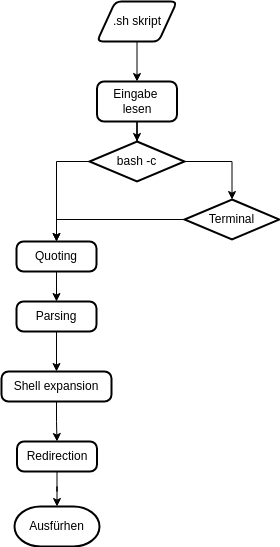
\includegraphics[scale=0.75]{shell_interpreter.png}
  \label{fig:shell}
\end{figure}
\pagebreak
Abbildung 1.1 beginnt von oben mit der Eingabe des Shell-Skripts. Das Shell skript kann neben Shell Commands, die auch in einer CLI ausgeführt werden können, Verzweigungen und Schleifen enthalten. Die Eingabe des Shellskripts wird Zeile für Zeile gelesen, entweder durch ein Terminal oder durch den Befehl \verb+bash -c+. 
Beide Eingabemethoden führen zu der ersten Phase des Shell-Interpreters, dass Quoting. Das Quoting arbeitet ähnlich wie ein Lexer. Hier werden alle Sonderzeichen entfernt, wie etwa Kommentare oder Backslashes. Sobbald das Quoting beendet ist entsteht ein String der lediglich aus Terminalsymbolen besteht und Nicht-Terminal Symbolen in Form von Datei- oder Variablennamen. Somit verbleiben nur Symbole, die im Zuge der Ausführung des Shellskripts eine Rolle spielen. 
Sobbald das Quoting abgeschlossen ist beginnt das Parsing. Diese Phase ähnelt zwar dem herkömmlichen Parsing aus dem Kompilierprozess, jedoch wird keine Zwischencode erzeugung aus dem Parsing erzeugt. Hier wird lediglich zwischen einfachen Commands und Commpound Commands unterschieden. Einfache Commands, sind etwa das Ausführen der Buitin-Shellprogramme \verb+ls+, \verb+wc+ oder \verb+mkdir+. Compound Commands bezeichnet alle Commands die zusätzliche Logik in das Shell-Programm bringen, mit etwa \verb+if+, \verb+while+ oder \verb+case+. In diesem Schritt wird festgestellt, ob zu jeden \verb+if+ etwa ein \verb+fi+ besteht. 
Der Übersetzungsprozess wird mit der Shell Expansion fortgesetzt und es werden in einem Kommando eingebundene relative Ausdrücke mit den Absoluten repräsentationen ersetzt. Beispielsweise würde in dem Ausdruck  \verb+echo ${pwd}+ das \verb+$pwd+ mit dem absoluten Pfad des aktuellen Verzeichnisses ausgetauscht.
Schlussendlich wird die Ausgabe des Shell-Skript über der die \verb+stdio+ libary ausgegeben. 
(https://www.gnu.org/software/bash/manual/bash.html#Shell-Operation)

In diesem gesamten Prozess wird lediglich die Shell Skriptsprache verwendet. Der Quellcode wird nicht von einer Hochsprache in eine Niedere-Sprache oder andere Hochsprache umgewandelt. Damit wird ein zentraler Unterschied zwischen einem Interpreter und einem Compiler deutlich. Es entsteht keine Repräsentation des Codes in einer andere Sprache. Von der Eingabe des Code bis zum Ergebnis des Programms, bleibt der Interpreter bei einer Sprache.

% @todo: Es soll deutlich werden welchen Begriff für das Programm gewählt werden soll. Vorher auch checken ob irgendwo ausser im Abstract Begriff Transpiler auftaucht.
  % Absatz: Zusammenfassende Unterscheidung zwischen Interpreter und Transpiler, Was sind gemeinsamkeiten und unterschiede von Transpiler und interpreter?
  % !!!HIER EVALUIEREN WELCHE ART, INTERPRETER/TRANSPILER!!!
  Ein One-Pass Compiler als Gestaltungsschema für die zu entwicklende Software ist nicht geeignet.
  
Zusammenfassend zeigen sich Ähnlichkeiten und Unterschieden zwischen einem Interpreter und einem Compiler. 

Zum einen durchlaufen beide die Phasen des Lexings und des Parsings. Bei dem Beispiel des Bash-Interpreters wurden andere Begriffe für diese Prozesse gewählt, wie etwa Quoting und Parsing, hingegen decken diese Prozessschritte, die eines Lexers oder Parsers ab. Es müssen sowohl Compiler, wie auch Interpreter den Quellcode erst um Kommentare, Leerstellen oder sonstige Nicht-Terminalsymbole bereinigen, die für Übersetzung nicht von Syntaktischer Relevanz sind. 

Zum anderen ist ein Interpreter ein Programm welches den Quellcode direkt ausführt. Ein Compiler hat zwischen dem tatsächlichen Ausführen des Programms, wesentliche Prozesschritte die je nach Ausprägung des Compilers unterschiedlich Ablaufen können.

   % - Erweiterung des Umfangs während der Laufzeit
   % - Trennung Laufzeit/Konzeptionsphase

   % - Hier erwähnen das eine geminsamkeit die definition von Grammatiken ist, dann überleiten zu Formale Grammatiken.
   % - Auch Entscheidung treffen was genau der Transpiler ist, Compiler oder Interpreter
   \pagebreak
   
   
	\subsection{Formale Sprachen und ihre Grammatiken}
	% Warum braucht ein Compiler eine Grammatik?
	In dem vorangegangen Kapitel wurden unterschiedliche Formen der Sprachinterpretation eines Computers vorgesteltt. Damit die Interpretation von Sprachen korrekt erfolgt, braucht ein Computer Regeln. Grammatiken beinhalten diese Regeln. Damit der Transpiler korrekt arbeitet wird eine definierte Grammatik benötigt. Nur so können die Prozessschritte der Lexikalischen- und der Syntatkischen Analyse korrekt erfolgen. Denn diese Schritte prüfen den eingegeben Quellcode auf seine grammartikalische Richtigkeit. Bevor also die Sprachliche Analyse erfolgen kann, sollte eine Grammatik angwendet werden.
	
	% Woraus besteht eine Grammatik
Um eine Grammatik anzuwenden, muss klar sein um welche Grammatik es sich handelt. Wiederum Klarheit zu erhalten um welche Grammatik es sich handelt, sollte bestimmt werden welche Art von Sprache beschrieben werden soll. Da es sich bei einem Transpiler um ein Computeprogramm handelt, ist die behandelende Sprache eine fromale Sprache. Eine formale Sprache unterscheidet sich von einer natürlichen Sprache in der Anwendungsform. Die Anwendung von solchen Sprachen dient der logisch präzisen Beschreibung von Ausdrücken und nicht der Kommunikation. Ein Beispiel für eine formale Sprache sind Programmiersprachen. Für eine Programmiersprache wird eine Grammatik benötigt die feste Regeln bestimmt. (introduction to formal languages and automata, S. 149ff.) Eine Grammatik besteht aus Variablen, Terminalsymbolen, einen Startsymbol und einer Produktion. Zusammengefasst in:
\begin{center}
\begin{equation}
G=(V,T,S,P)
\end{equation}
\end{center}
Wobei \verb+V+ für Variablen, \verb+T+ für Terminale, \verb+S+ für Start und \verb+P+ für Produktion steht. Dabei ist \verb+S+ ein Teil von \verb+V+. (introduction to formal languages and automata, S. 31ff.) Für Variablen wird häufig auch der Begriff von Nicht-Terminalsymbolen verwendet.
% Welche Typen von Grammatiken gibt es? Chomsky Hierarchie
Grammatiken lassen sich weiter durch die Chomsky Hierarchie spezifizieren. Normane Chomsky unterteilt Grammatiken in vier Ebenen. Ebene null beschreibt unbeschränkte, Ebene eins kontextsensitve, Ebene zwei kontextfreie und Ebene drei reguläre Grammatiken.(https://hpi.de/friedrich/teaching/units/grammatiken.html) 
\pagebreak
Wobei unbeschränkte Grammatiken immer gegeben sind, solange mit einer Produktion auch mindestens ein nicht-Terminalsymbol beschrieben wird. Das ist bei Grammatiken von Programmiersprachen der Fall. Denn es wird beispielsweise bei der Variablen-Deklaration folgende Form unterstellt:

\begin{center}
\begin{equation}
S \to TB;
\end{equation}
\begin{equation}
T \to int | char | float
\end{equation}
\begin{equation}
B \to AD
\end{equation}
\begin{equation}
A \to A...Z|a...z
\end{equation}
\begin{equation}
D \to 0...9|D
\end{equation}
\end{center}
 
Kontextsensitiv ist die Grammatik einer Programmiersprache ebenfalls. Mit der beschriebenen Grammatik ist folgender Ausdruck zulässig.
% Beispiel überprüfen----------------
\begin{verbatim}
int identifier;
\end{verbatim}
% -----------------------------------
Nicht zulässig ist hingegen.
% Beispiel überprüfen---------------
\begin{verbatim} 
identifiert int; 
\end{verbatim}
% ---------------------------------
Somit ist die Grammatik einer Programmiersprache kontextsensitiv. 
Bei der deklaration einer Variable ist es eindeutig das der Kontext der Terminalsymbole zu den Nicht-Terminalsymbolen zu berrücksichtigen ist. Jedoch kann auch eine mehrdeutigkeit entstehen. Zusätzlich sollte deshalb auf der linken Seite genau ein Nicht-Terminalsymbol stehen. Somit ist die definierte Grammatik ebenfalls Kontextfrei. 
Weiterhin kann in diesem Beispiel die Produktion als Terminalfolge aufgebaut werden. Etwa mit: 

\begin{center}
\begin{equation}
S \to TB \to int | double | float B \to AD \to A...Z|a...z D \to 0...9|D;
\end{equation}
\end{center}

Jedoch ist dieser Ausdruck damit nicht Regulär. Durch den Rekursiven Aufruf am Ende kann kein endlicher Automat erzeugt werden. Die Grammatik bleibt also höchstens von Typ 2.

	% Grammatik Reguläre Ausdrücke einordnen
	% Grammatik PL/I einordnen
	
	% Wie werden Grammtiken in einem Transpiler Programm verwendet?
Die bisher definierten Grammatiken sind in dem Sinne von Bedeutung, weil die Lexikalsiche und Syntaktische Analyse des Transpilers aus einer solchen Grammatik erzeugt werden. Mithilfe des Parser-Generator Programms JavaCC wird eine Grammatik definiert aus der ein Parser erzeugt wird, der eben nur definierte Ausdrücke zulässt. Für PL/I bedeutet dies das die aktuelle Sprachnorm für den Parser definiert werden muss. Die aktuellste Sprachnorm wird durch IBM definiert. In der PL/I Language Referenz werden jegliche zulässige Ausdrücke definiert. Da hingegen bisher keine vollständige Grammatik definition in From eines Parsers besteht der öffentlich zugänglich ist muss die Grammatik eigenhändisch definiert werden. Schlussendlich erzeugt der Compiler-compiler JavaCC die Module für die Lexikalische und Syntaktische Analyse. Weshalb Kapitel 1.5 die in diesem Kapitel definierte Theorie praktisch darstellt.^
    % - Theoretischer Abriss
   % - Einordnung der resultate der PA 4
	%- PL/1 Syntax Wo zu finden? Welche Version der Sprache? 
%	- Reguläre Ausdrücke Syntax, Beispiel einer Grammatik die ich mit verwende, Typ einer Grammatik
  %  - Literatur
	%    - Chomsky Hierarchie Bücher
	%    - https://www-igm.univ-mlv.fr/~berstel/LivreCodes/Codes.html
   %  - Woraus besteht eine Grammatik?
  %   - Wie lassen sich Grammatiken der Komplexität nach anordnen?
   %  - Chomsky Hierarchie
   %  Erst Chomsky Hierachier, dann nach Komplexität einordnen und am Beispiel von Regulären Ausdrücken und PL/I Grammatik einführen.
     
	\subsection{Anwendung von Formalen Grammatiken in JavaCC}
  %   - Beschreibung von formalen Grammatiken, als Input für den Compiler Compiler JavaCC.
    % - Entwurf von Java Klassenhierachie für PL/I Datentypen
   %  - Übersetzung von Kontrollstrukturen und komplexeren Programmabläufen
    %   Wie kann JavaCC die formale Beschreibung der Grammatik in einen Parser Umsetzen?


\section{Technisches Vorgehen}
\subsection{Techstack}
Um den Transpiler weiter zu entwickeln sind Schritte notwendig die, die Qualität des bestehenden Projektes erhöhen. Diese Schritte sind einerseits die Verbesserung der Projektstruktur und andererseits die Handhabung von Bugs und Fehlern.

Die Ursprüngliche Version des Transpilers nahm die Native Projektstruktur von Eclipse als Vorlage. Diese Projektvorlage brachte jedoch einige negative Aspekte mit sich. Mit dieser Struktur war es schwer das Projekt zu importieren und erfolgreich PL/I-Code zu transformieren. Das erschwerte den Benutzern den Zugang zu dem eigentlichen Projekt.
Zurückzuführen ist dies auf das fehlenden Dependency Management. In der Ursprünglichen Version des Transpilers musste der Benutzer selbst herausfinden welche Software dieser benötigt um das Programm zu starten. In den meisten Fällen durch Fehlermeldungen welche darauf schließen lassen konnten das eine Dependency fehlt. Dieser Umstand ergibt eine Hürde, welche den Einstieg in die Umwandlung erschwerte. 
Dieses Problem wurde gelöst in dem das Software Projektmanagement Werkzeug Maven eingesetzt wurde. Maven kann mithilfe des Project-Object-Model (POM) Dependecies lösen in dem benötigte Softwared beim kompilieren installiert wird. Der Benutzer kann nun entweder mithilfe des Maven Commandline-Interface (CLI) das Projekt aufbauen, oder einfach in Eclipse oder einer selbstgewählten IDE importieren.
Ein weiterer Vorteil den Maven liefert ist die vordefinierte Projektstruktur. Mavens Projektstruktur liefert zwei gespiegelte "src" Ordner, welche je den Quellcode enthalten und die dazugehörigen Tests. Diese Struktur wurde erweitert. Es wurde die Projektstruktur in Module unterteilt. Jeder Modul-Ordner beinhaltet Klassen in denen sich die funktionalität des Moduls wiederspiegelt. Die Module werden in den Basepackages Zusammengefasst. Bei der Auswahl der Module sollte der Prozess des Transformierens deutlich werden, entsprechend erfolgt die Namensgebung nach den Prozesschritten: Lexikalische Analyse, Syntaktische Analyse, Syntaktische Synthese. Neben den Hauptprozessschritten, sind die Nebenprozess die Verarbeitung der Symboltablle und die Fehlerbehandlung, welche Ebenfalls als Module geordnet sind. Diese Ordnung führt zu einer einfachen Übersicht der verschiedenen Prozesse.

%- Maven -> Dependency Management
%- Testing -> JUNit Tests
%- Platform -> Spring
%- Compiler Compiler -> JavaCC

\subsection{Architektur} 
% Abstractes UML einbinden
%--> UML Diagramm Zielbild einfügen, dynamisches Diagramm
%- Wie sind die Module momentan gebaut
%- Wie sind Module zueinander abhängig
%- Wie wird es erweitert

%Wie Benutze ich den Transpiler:
%Bausteine
%- Software Architektur
	%- Planen mithilfe eines UML
	%- UX Design 
    %    - zweite Diagramm, des Benutzerfluss
    %    - wie Benutzung abläuft
	%	- Website?
	%	- Docker Container?
%- Fehlertracking
%- Struktuierung des Programms, sodass ein Benutzer es selbständig erweitern kann

\subsection{Aspektorientierte Programmierung}
%- Wie funktioniert Aspektorientiert Programmierung?
%	- Wie Löse ich mit Aspektorientierter Programmierung konkrete Probleme?
%- JavaBeans
%- Spring
%	- Wie setzt Spring Aspektorientierte Programmierkonzepte ein?
 
\subsection{Module des Transpilers}
\subsubsection{Compiler-Compiler}
\paragraph{Scanner}
\paragraph{Lexer}
\paragraph{Parser}
\subsubsection{Symboltable}

\subsubsection{Mapper}

\subsubsection{Error-Handling}

\subsection{Testing und Integration}
%1. Transpiler wird getestet
%1.1 Testen der Methoden von Lexer, Parser usw. (Bsp.: Kann dieses Zeichen verarbeitet werden?)
%1.2 Baum testen auf Korrektheit

%2. Transpilieren wird getestet
%2.1 Output des transpilierten Pl/1 Codes im Verhältnis zum Pl/1 Code testen.

%3. Der Transpilierte Code wird getestet
%- Wie wird PL/1 Code Native getestet
%- Funktioniert der Java Code richtig

%4. Performance Test (erst am ende)

\subsection{Fehlerbehandlung}
Um dem Benutzer die Bediengung während der Laufzeit zu erleichtern, wurden Selbstgewählte Fehlermeldungen implementiert. Diese Fehlermeldungen sollen den Benutzer der Software in eine Feedback schleife bringe welche klare Anweisung zur Bediengung gibt. In der usprünglichen Version des Transpilers wurde dem Benutzer lediglich die von Java geworfenen Fehler in der Konsole ausgegeben. Die Fehlermeldung"IndexOutOfBounds", ließ dabei nicht darauf schließe das der Transpiler die PL/I Datei zum lesen nicht findet. Eine solche Fehlermeldung führt erneut dazu, dass der Benutzer sich selbst um die Lösung des Problems kümmern musste und somit einer weiteren Hürde begenete.
Eben für dan Fall das die Datei nicht gelesen werden kann, wurde eine Exception geschrieben. Die Exception "PliFileNotFound", beschreibt dem Benutzer die Ursache des Problems und nennt auch ein etwaaigen Lösungsvorschlag. Es exstieren in der neusten Version einige Exceptions die in der folgenden Tabelle näher Beschrieben werden.

...Tabelle mit Exceptions...

Fehlerbehandlung spielt besonder im Zusammenhang mit der Lexikalischen Analyse eine Rolle. Um zu gewährleisten das die Transformation korrekt albläuft braucht es der formalen PL/I Grammatik enstrpechend richtigen PL/I Code als Eingabe. Eine nicht behandlung hätte zur Folge das das Programm entweder eine Fehlerhafte Ausgabe produziert, oder Fehlschlägt. Dies soll vermieden werden.

\section{Technische Spezifikation}
	\subsection{Ausführung des Transpilers}
		\subsubsection{Transformationsmöglichkeiten}
		%Toleranzspielräume:...Einfach, Genau, Präzisse
		\subsubsection{Umwandlung von Datentypen}
		\subsubsection{Umwandlung von Prozeduren}
	\subsection{Optimierung}
		\subsubsection{Performance und Benchmarks}
		\subsubsection{Testing}
